\section{Comparison Using FA4-Reported Baseline Performance}
\label{app:fa4_baselines}

Section~\ref{sec:experiments} reports cuDNN and FA4 throughput measured on our hardware. In practice, minor system-level differences (driver versions, thermal conditions, clock frequencies) can affect absolute TFLOPS. Therefore, we additionally compare AVO against the cuDNN and FA4 numbers published in the FA4 paper~\citep{zadouri2026flashattention4}. Figure~\ref{fig:mha_official} presents this comparison.

\begin{figure}[h]
  \centering
  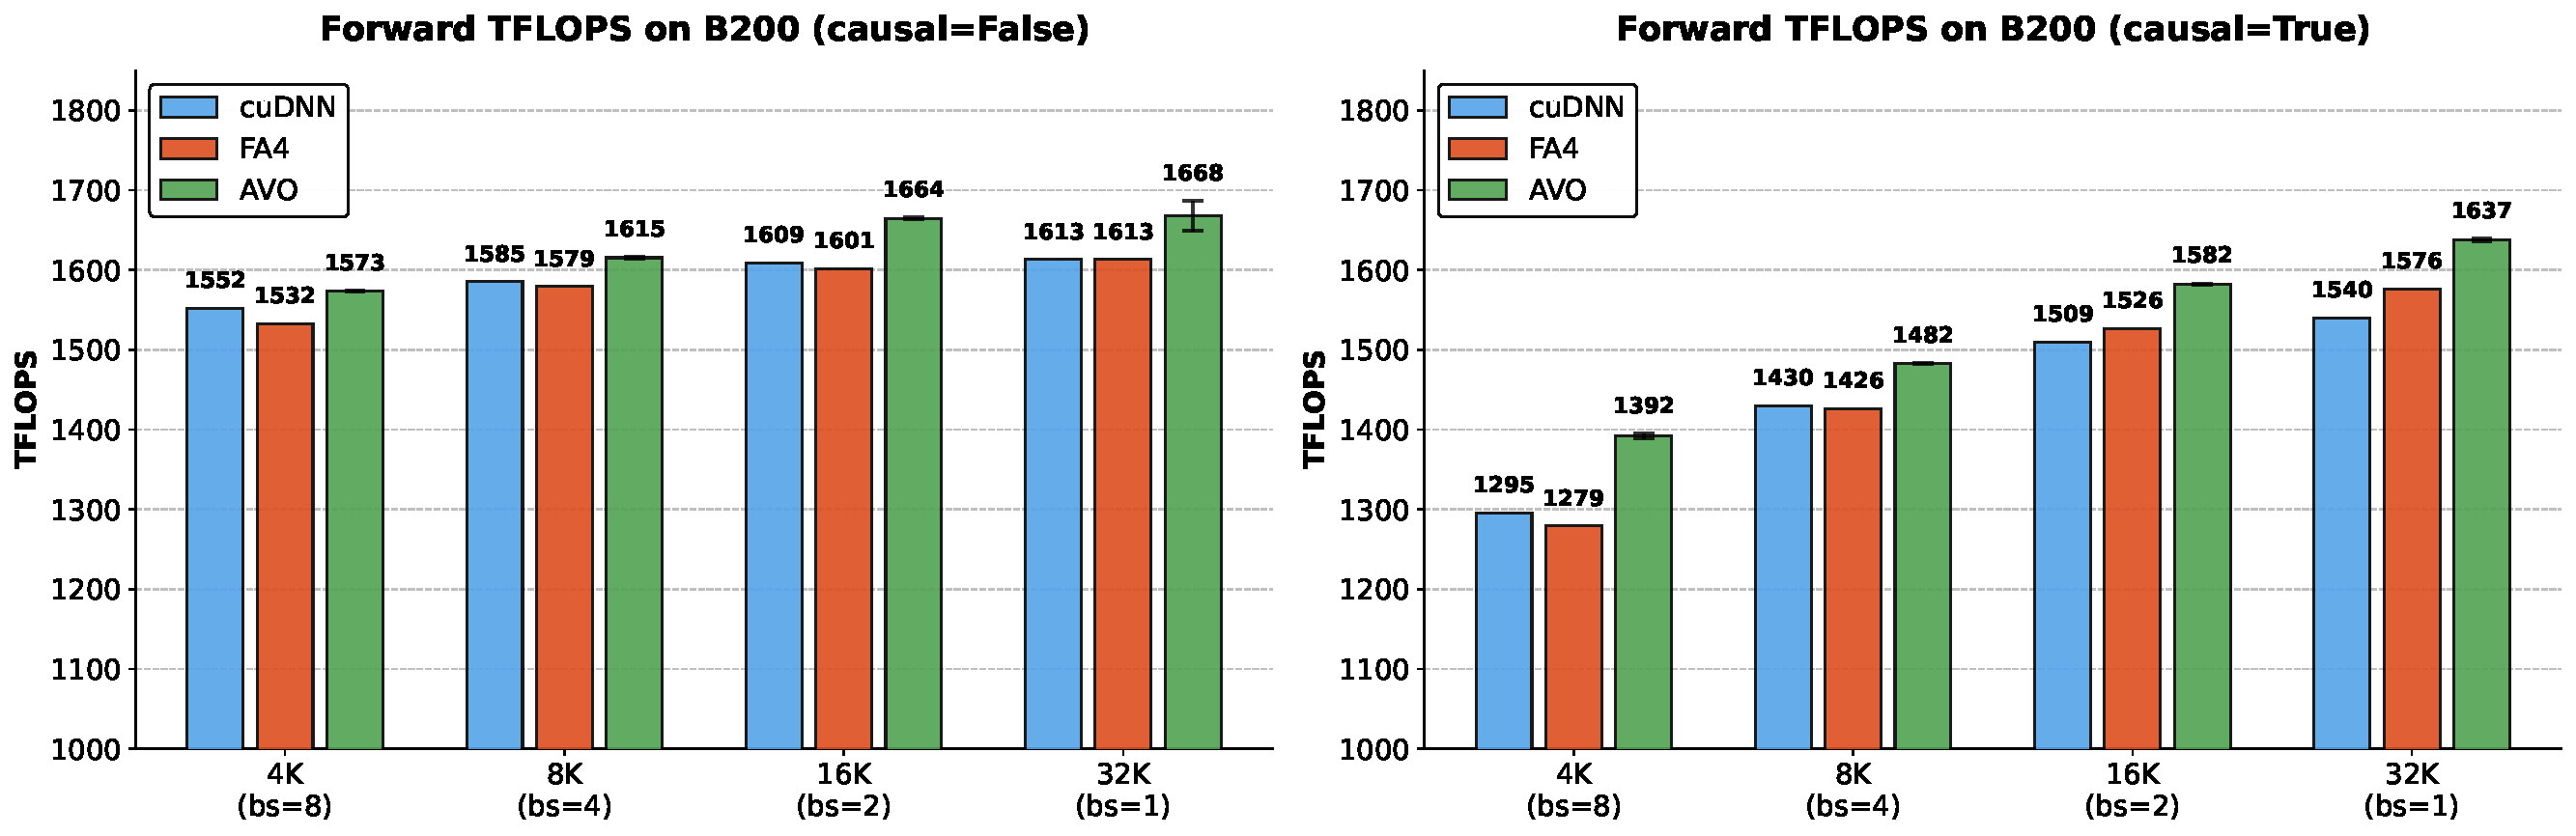
\includegraphics[width=\textwidth]{figures/mha_performance_official.pdf}
  \caption{Multi-head attention forward-pass throughput (TFLOPS) on NVIDIA B200, comparing AVO (measured on our hardware) against cuDNN and FA4 baseline numbers as reported in the FA4 paper~\citep{zadouri2026flashattention4}. Head dimension 128, 16 heads, BF16. Left: non-causal. Right: causal.}
  \label{fig:mha_official}
\end{figure}

On non-causal attention, AVO outperforms the FA4-reported baselines across all configurations, with gains of $+1.4\%$ to $+3.4\%$ over cuDNN and $+2.3\%$ to $+3.9\%$ over FA4.
On causal attention, AVO achieves $+3.6\%$ to $+7.5\%$ over cuDNN and $+3.7\%$ to $+8.8\%$ over FA4, with the largest gains observed at shorter sequences (bs=8, seq=4096).
These results are broadly consistent with the comparisons in Section~\ref{sec:experiments}.